\subsection{Profilo utente}
La schermata del profilo utente è accessibile cliccando sull'icona dell'utente posizionata in alto a destra nella barra degli strumenti, come specificato nel paragrafo RIFERIMENTO. Da questa schermata, gli utenti possono visualizzare e modificare le proprie informazioni personali, nonché accedere alle preferenze dell'utente per apportare eventuali modifiche.\\
La schermata del profilo utente è composta da tre schede principali:
\begin{itemize}
    \item Profile;
    \item Notification history;
    \item Change password.
\end{itemize}
\begin{figure}[H]
    \centering
    \fbox{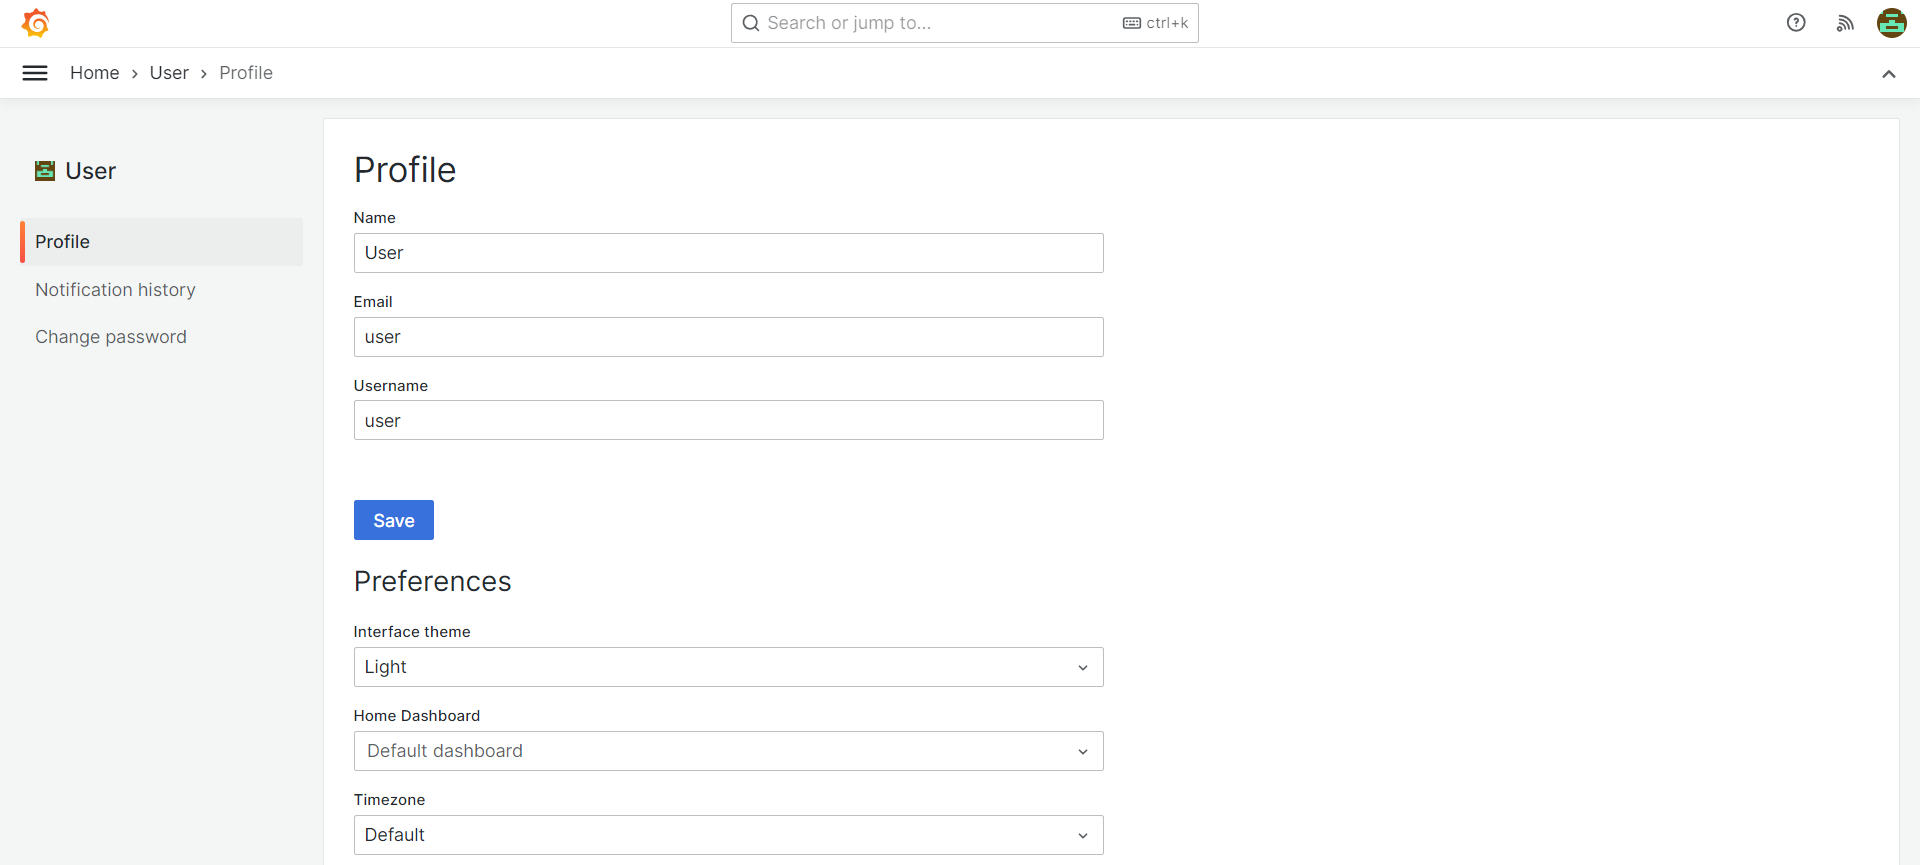
\includegraphics[width=16cm]{../Images/ManualeUtente/Light/schermata_profilo_utente.png}}
    \caption{Schermata del profilo utente}
    \label{fig:my_label}
\end{figure}

\subsubsection{Profile}
La schermata dedicata al profilo utente consente di visualizzare e modificare le informazioni personali dell'utente. In particolare è possibile visualizzare e modificare Nome, Email, ed Username. Una volta apportate le modifiche desiderate, è possibile confermarle cliccando sul pulsante "Save".\\
Sono presenti altre tre sotto-sezioni:
\begin{itemize}
    \item Preferences;
    \item Organizations;
    \item Sessions.
\end{itemize}
\paragraph{Preferences}
La sezione "Preferences" consente di modificare le seguenti preferenze:
\begin{itemize}
    \item tema dell'interfaccia;
    \item dashboard predefinita (Home dashboard);
    \item fuso orario;
    \item inizio della settimana;
    \item lingua;
\end{itemize}
Una volta modificata la scelta tramite un pratico menù a tendina, è possibile confermare le modifiche cliccando sul pulsante "Save".\\
\paragraph{Organizations}
La sezione "Organizations" consente di visualizzare le organizzazioni a cui l'utente appartiene. Per ogni organizzazione è possibile visualizzare il nome e il ruolo dell'utente all'interno di essa.
\begin{figure}[H]
    \centering
    \fbox{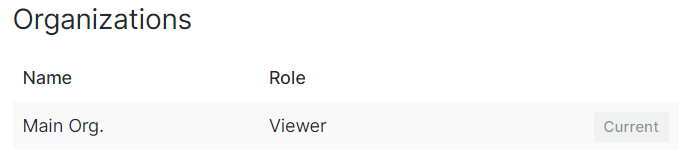
\includegraphics[width=10cm]{../Images/ManualeUtente/Light/profile_organizations.png}}
    \caption{Profilo utente sezione "Organizzazioni"}
    \label{fig:my_label}
\end{figure}
\paragraph{Sessions}
La sezione "Sessions" consente di visualizzare le sessioni attive dell'utente. Per ciascuna sessione è possibile visualizzare la data e l'ora dell'ultimo accesso, l'indirizzo IP, nonché il browser e il sistema operativo utilizzati. Attraverso un pulsante dedicato, è possibile terminare la sessione desiderata.
\begin{figure}[H]
    \centering
    \fbox{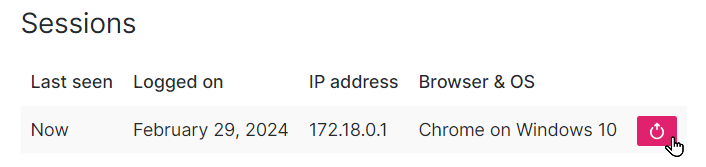
\includegraphics[width=10.5cm]{../Images/ManualeUtente/Light/profile_sessions.png}}
    \caption{Profilo utente sezione "Sessioni"}
    \label{fig:my_label}
\end{figure}

\subsubsection{Notification history}
La schermata "Notification history" consente di visualizzare la cronologia delle notifiche degli errori o delle avvertenze. Per ciascuna notifica è possibile visualizzare la data e l'ora, il tipo di notifica e, se presente il messaggio corrispondente.
\begin{figure}[H]
    \centering
    \fbox{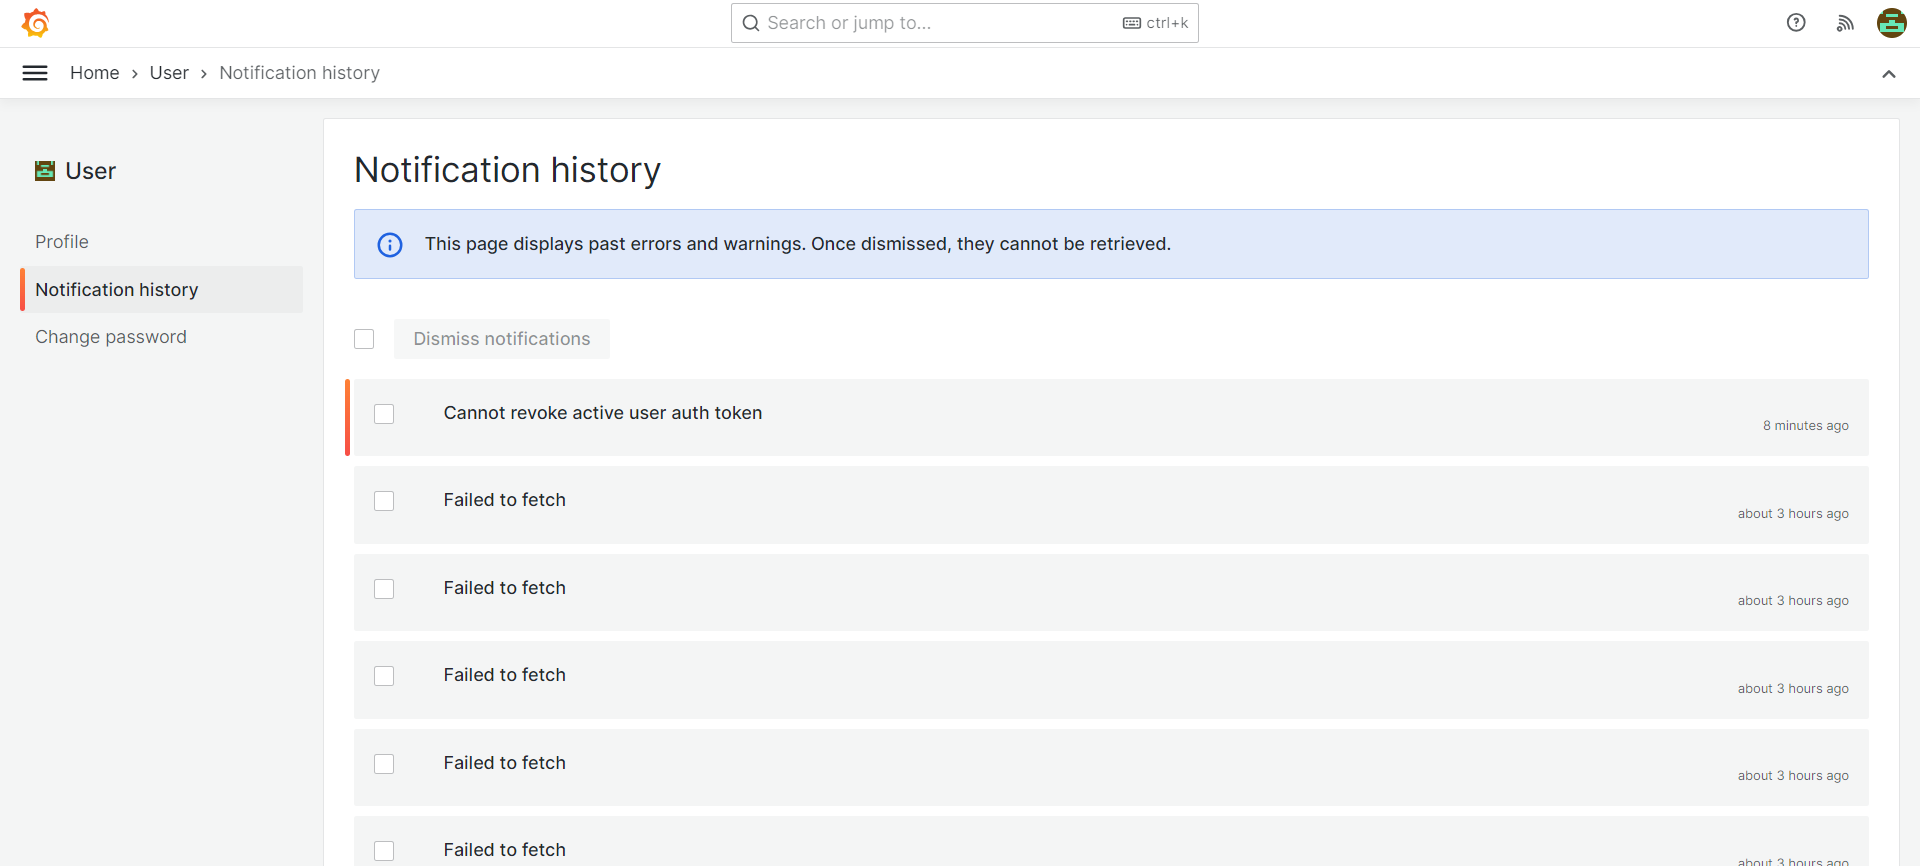
\includegraphics[width=16cm]{../Images/ManualeUtente/Light/notifications_history.png}}
    \caption{Schermata "Cronologia delle notifiche"}
    \label{fig:my_label}
\end{figure}
È possibile selezionare una o più notifiche e cliccando sul pulsante "Dismiss notifications" è possibile eliminare le notifiche selezionate (una volta cancellate non sarà più possibile recuperarle).
\begin{figure}[H]
    \centering
    \fbox{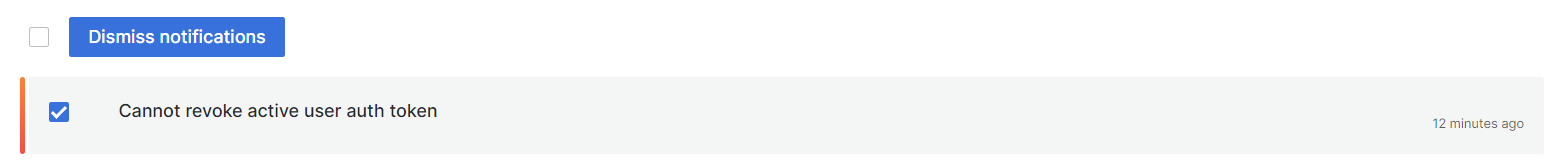
\includegraphics[width=12cm]{../Images/ManualeUtente/Light/dismiss_notificaitions.png}}
    \caption{cancellare le notifiche}
    \label{fig:my_label}
\end{figure}

\subsubsection{Change password}
La schermata "Change password" consente di modificare la password dell'utente. Per modificare la password è necessario inserire la password corrente, la nuova password e confermare la nuova password. Una volta inserite le informazioni richieste, è possibile confermare le modifiche cliccando sul pulsante "Change Password" o, in alternativa, annullare le modifiche cliccando sul pulsante "Cancel".
\begin{figure}[H]
    \centering
    \fbox{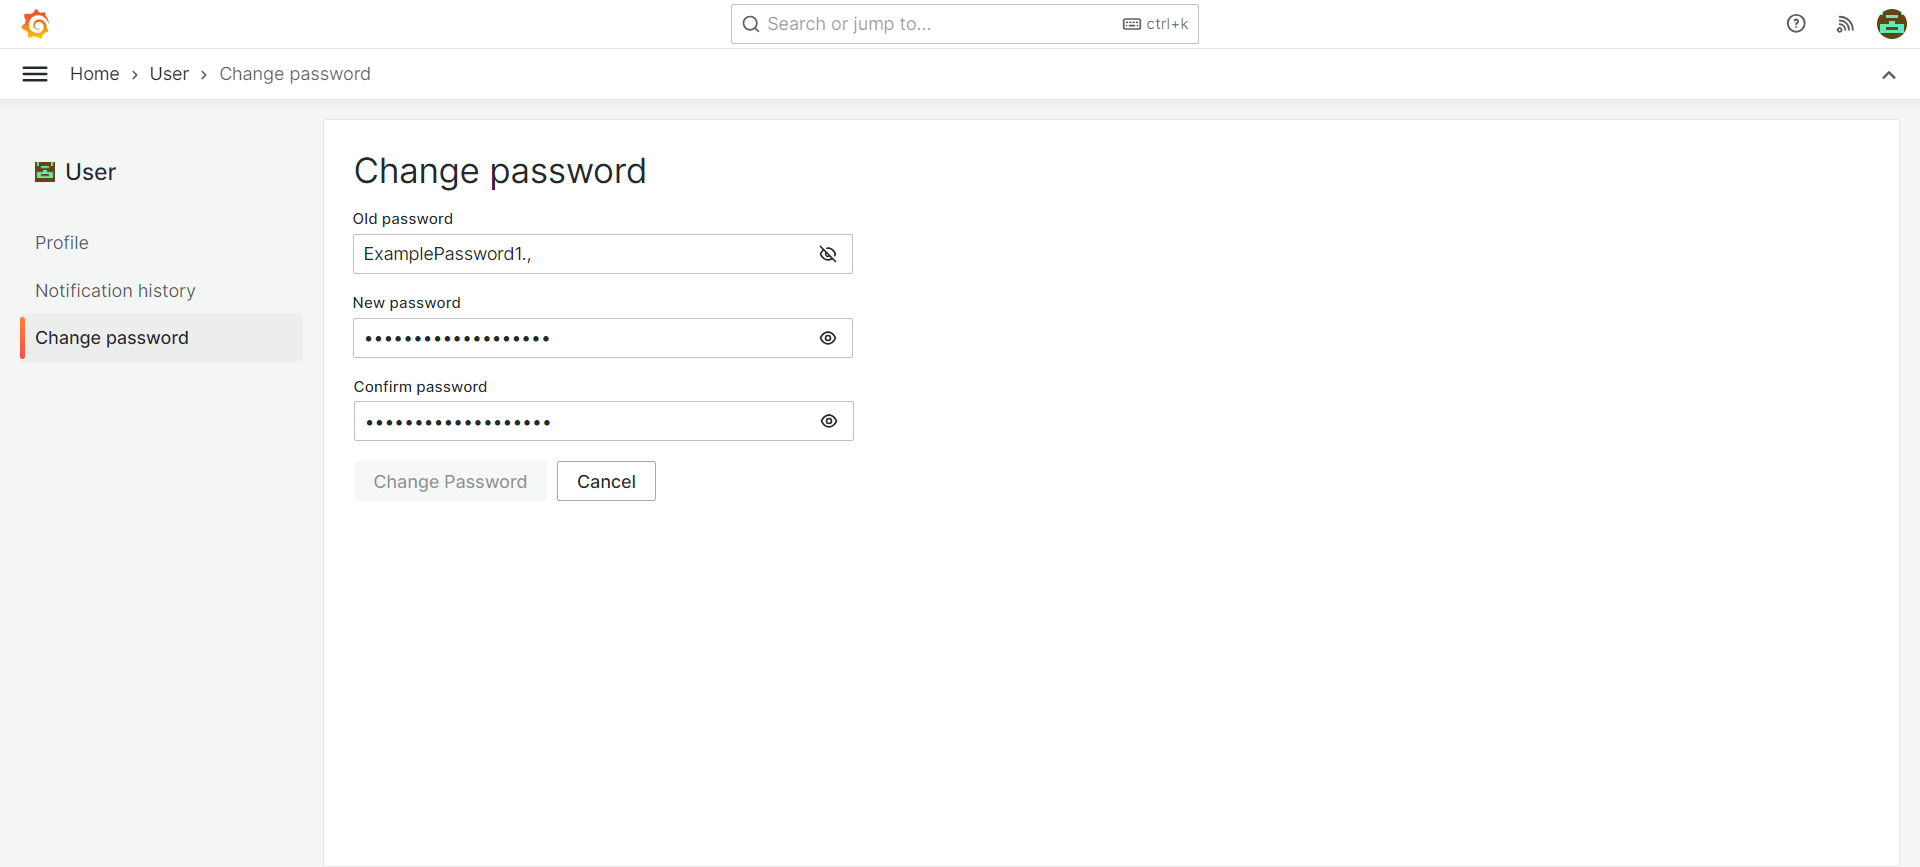
\includegraphics[width=16cm]{../Images/ManualeUtente/Light/cambia_password.png}}
    \caption{Schermata "Cambia password"}
    \label{fig:my_label}
\end{figure}
Cliccando sull'icona rappresentante un occhio, è possibile visualizzare la password inserita e, cliccando nuovamente sull'icona, è possibile nascondere la password.
\begin{figure}[H]
    \centering
    \fbox{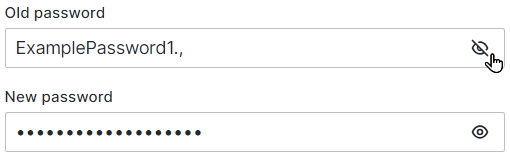
\includegraphics[width=8cm]{../Images/ManualeUtente/Light/visualizza_password.png}}
    \caption{Visualizzare la password inserita}
    \label{fig:my_label}
\end{figure}
\begin{center}
    \textbf{Attenzione}: la password inserita nell'immagine è a puro scopo illustrativo e non rappresenta la password reale dell'utente.\\
\end{center}
 